\subsection{Data collection protocol}

WhiteTiger trajectories are collected through human teleoperation on physical robot platforms. Human teleoperation is widely used for action-labeled robot demonstrations in fixed-base, bimanual, in-the-wild, and mobile manipulation settings~\cite{mandlekar2018roboturk,sharma2018mime,zhao2023aloha,fu2024mobilealoha,khazatsky2024droid}. The released corpus excludes scripted rollouts, simulation trajectories, and internet-sourced robot videos. Each episode records an operator controlling a real robot to complete a requested manipulation task under a specified scene configuration.

Task annotations are provided manually by the task requester before collection. The task label or instruction therefore encodes the intended scene setup, object set, target state, and manipulation procedure rather than a post hoc caption inferred from logs. This protocol aligns language supervision with the collection requirement and supports conditioning by task semantics during model training.

Observation and action spaces remain platform-specific across the 14 robots. Camera count, viewpoint, camera model, proprioceptive fields, and sensor configuration depend on the platform and collection setup. Action representations may include arm joints, end-effector commands, gripper states, dexterous-hand controls, mobile-base commands, or other platform-specific dimensions. WhiteTiger preserves these native schemas inside a standardized dataset interface, avoiding artificial control-space collapse across embodiments with different physical constraints.

\subsection{Skill taxonomy}

WhiteTiger covers 64 manipulation skills across 6195 tasks. The taxonomy groups task executions by reusable action semantics rather than treating every task string as an isolated category. Skill labels span object acquisition, placement, handover, articulated-object interaction, contact-driven motion, tool use, material manipulation, and navigation-related actions.

Figure~\ref{fig:skill-taxonomy} organizes the 64 skills into seven action-semantic categories. The taxonomy provides an intermediate representation between task names and raw trajectories. A single task may require multiple skills, while a single skill may appear across objects, scenes, and robot embodiments. Category counts denote defined labels rather than occurrence frequencies, thereby characterizing behavioral coverage without conflating taxonomy size with sampling density.

\begin{figure}[t]
\centering
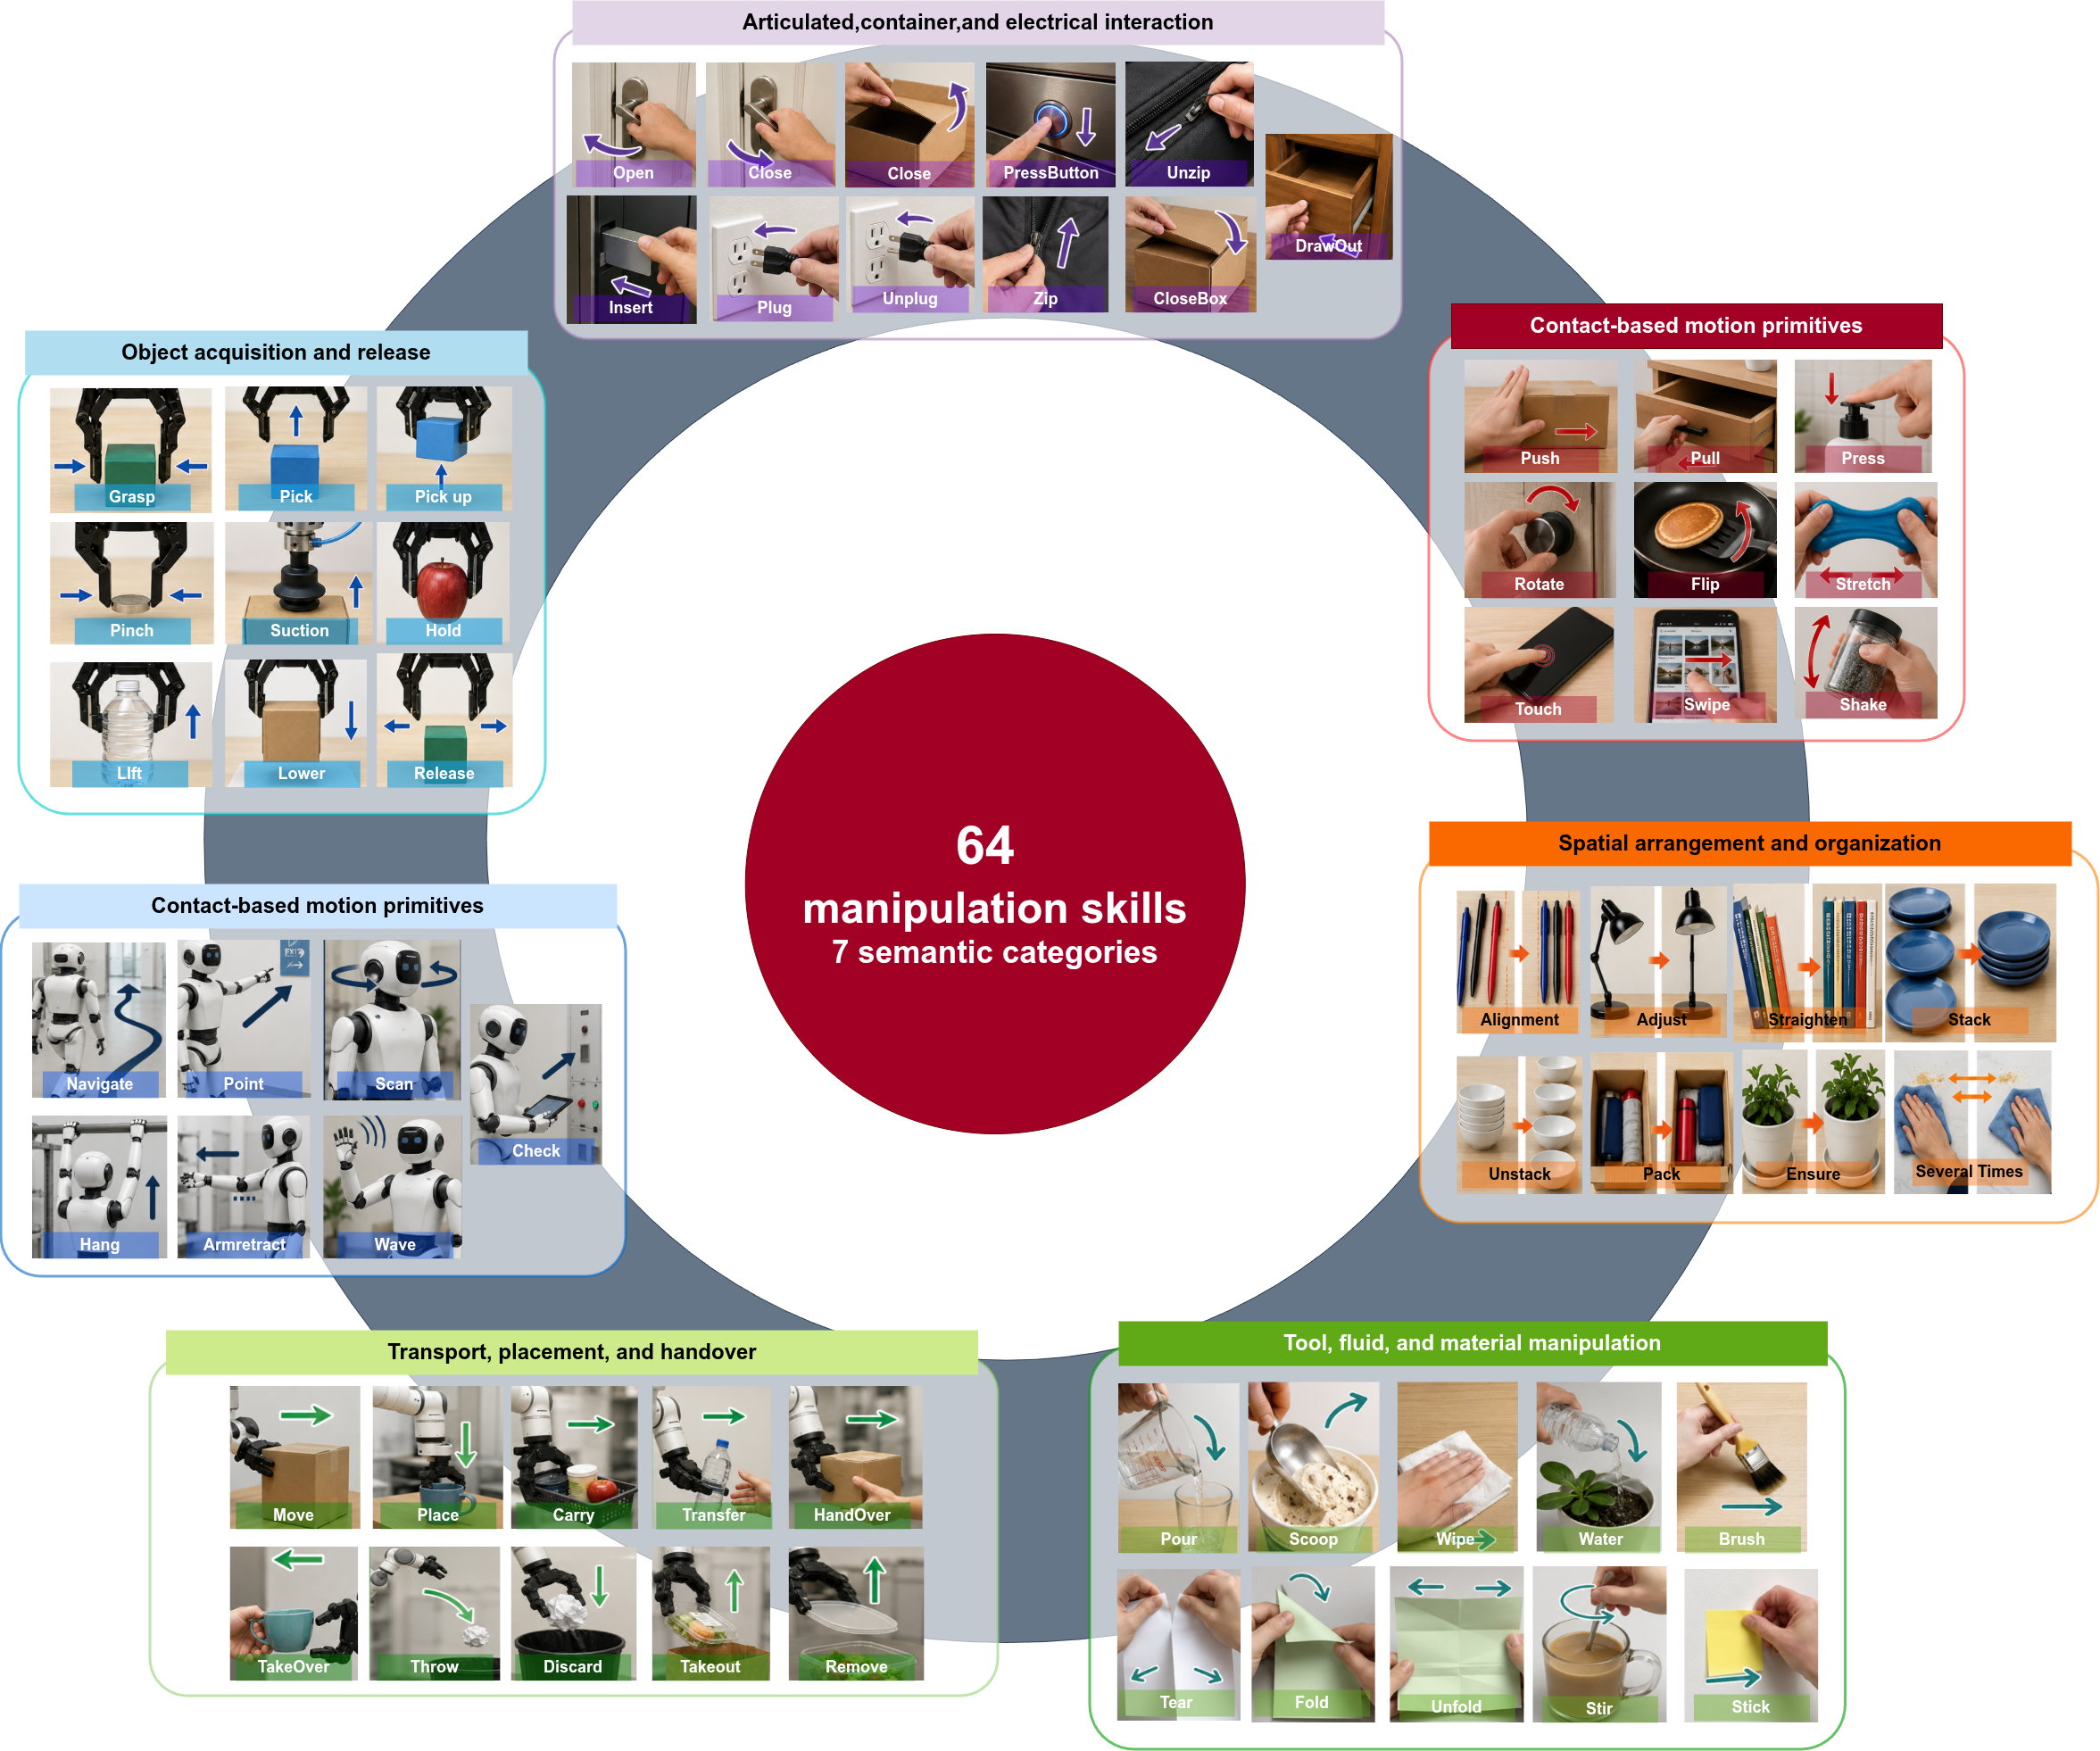
\includegraphics[width=0.75\textwidth]{figures/技能分类-rearranged.png}
\caption{Skill taxonomy of WhiteTiger. The 64 manipulation skills are grouped into seven action-semantic categories used during data collection and annotation. Each skill label can occur across different objects, scenes, and robot embodiments, while a single task may comprise multiple skills. Category counts denote defined skill labels rather than dataset occurrence frequencies.}
\label{fig:skill-taxonomy}
\end{figure}

\subsection{Scenario and task coverage}

WhiteTiger covers manipulation scenarios organized into five categories: household service, retail and pharmacy, catering service, industrial manufacturing, and other general-purpose settings. Figure~\ref{fig:scenario-task-coverage} reports the task distribution across these scenario categories.

Scenario coverage determines how policy learning encounters variation in environment layout, object affordance, task objective, and interaction context. WhiteTiger contains 6195 tasks spanning short-horizon primitives and longer task chains. Many tasks compose lower-level manipulation skills such as grasping, placing, pushing, pulling, handing over, inserting, pressing, opening, closing, sorting, and arranging. This compositional structure supports direct action prediction, skill abstraction, temporal segmentation, and analysis of how reusable sensorimotor routines transfer across physical contexts.

Task duration provides a quantitative view of temporal structure. For each task, the mean trajectory duration is computed over all associated trajectories and assigned to a duration bin. Figure~\ref{fig:task-duration} summarizes the resulting task-level duration distribution, exposing the range of control horizons represented by short local behaviors and extended multi-stage interactions.

% TODO: Regenerate scenario_task_coverage3.png and task_duration_distribution2.png using the expanded 6195-task dataset inventory.
\begin{figure}[t]
\centering
\begin{subfigure}[t]{0.46\textwidth}
    \centering
    \includegraphics[width=\linewidth]{figures/scenario_task_coverage3.png}
    \caption{Scenario-level task coverage.}
    \label{fig:scenario-task-coverage}
\end{subfigure}
\hfill
\begin{subfigure}[t]{0.47\textwidth}
    \centering
    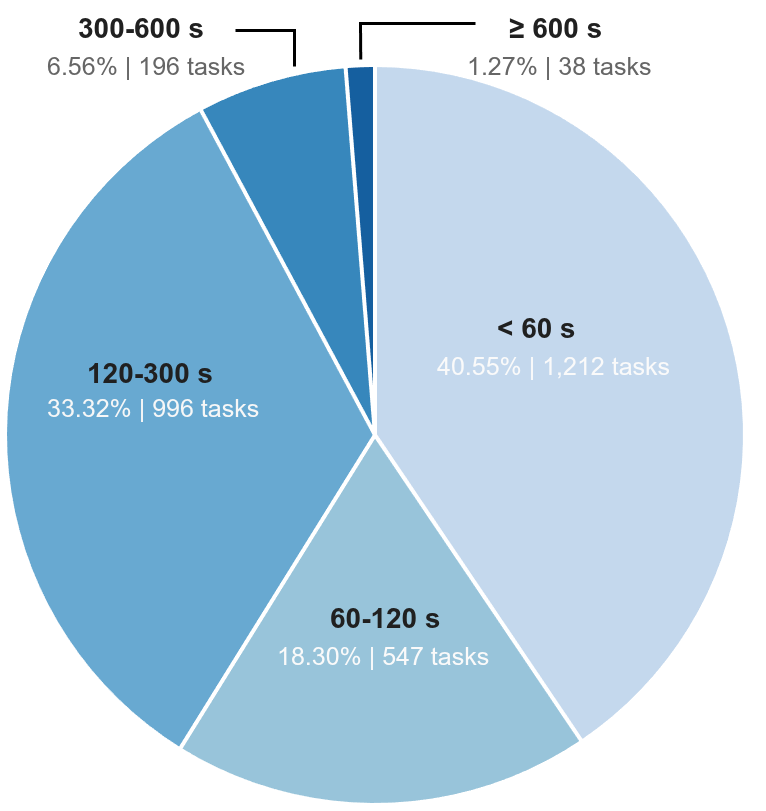
\includegraphics[width=\linewidth]{figures/task_duration_distribution2.png}
    \caption{Task-level mean trajectory duration.}
    \label{fig:task-duration}
\end{subfigure}
\caption{Task coverage and temporal diversity of WhiteTiger. The left panel reports task distribution across five scenario categories, and the right panel reports task-level mean trajectory duration.}
\label{fig:WhiteTiger-task-coverage}
\end{figure}

The duration distribution shows that WhiteTiger includes local manipulation behaviors and extended multi-stage interactions. Duration does not fully determine task complexity, but it exposes the control horizons and temporal variation that affect policy learning, event annotation, and open-loop evaluation.

\subsection{Event-level temporal annotations}

WhiteTiger provides event-level temporal annotations alongside dense observation-action trajectories. Events are semantic temporal milestones rather than actuator-state labels. An event marks localized task progress, including subgoal achievement, task-phase transition, contact transition, alignment state, boundary crossing, or object-state change. Gripper and dexterous-hand opening or closing can define events in contact-rich manipulation, but many physical interaction states are not directly recoverable from hand actuation alone.

In cloth folding, the lifting peak marks the transition from lifting to folding. In container placement, the rim-clearing frame marks an object crossing a spatial boundary. In insertion, pre-insertion alignment and fully seated states mark distinct physical constraints. In bimanual handover, the transfer pose and load-transfer moment define interaction states between two effectors. These examples show that WhiteTiger events encode task progress and object-state transitions beyond low-level commands.

Each event annotation includes an episode index, frame index, event label, event type, and annotation source. Event types include gripper events, contact events, motion events, alignment events, boundary-crossing events, object-state events, handover events, and deformation-related events. The visual frame, robot state, and robot or end-effector pose at an event can be used as attributes by methods requiring keyframe or keypose targets. The unified event interface preserves dense trajectory supervision while exposing the temporal structure required for event-conditioned policies and phase-aware evaluation.

\begin{table}[t]
\centering
\caption{Examples of event-level temporal annotations in WhiteTiger. Events are defined as task-dependent semantic milestones rather than only gripper or dexterous-hand state changes.}
\label{tab:event-keyframe-examples}
\footnotesize
\setlength{\tabcolsep}{4pt}
\renewcommand{\arraystretch}{1.08}
\begin{adjustbox}{max width=\textwidth}
\begin{tabular}{lll}
\toprule
Task type & Example event & Event meaning \\
\midrule
Cloth folding & \texttt{lift\_peak} & Cloth reaches the highest lifting point before folding \\
Container placement & \texttt{rim\_cleared} & Object passes over the container boundary \\
Insertion & \texttt{pre\_insert\_aligned} & Object is aligned with the insertion target \\
Bimanual handover & \texttt{handover\_pose\_reached} & Object reaches the transfer pose between two arms \\
Stacking & \texttt{stack\_stable} & Object remains stable after placement \\
Articulated-object interaction & \texttt{drawer\_fully\_open} & Drawer or lid reaches the fully open state \\
Pouring & \texttt{max\_tilt\_reached} & Container reaches the maximum pouring angle \\
Flexible-object insertion & \texttt{compression\_peak} & Soft object reaches maximum compression during insertion \\
\bottomrule
\end{tabular}
\end{adjustbox}
\end{table}

Event frames can serve as sparse targets for next-event prediction, waypoints or subgoals for goal-conditioned policies, boundaries for skill segmentation and hierarchical policy learning, anchors for event-to-event action generation, intermediate visual targets for future-state prediction, progress signals for value-guided policy improvement, stage rewards for reward shaping, and diagnostic checkpoints for phase-aware evaluation. The annotations are therefore algorithm-agnostic temporal supervision for goal-oriented robot learning rather than labels tied to a single reinforcement-learning formulation.

\subsection{Robot platform composition}

WhiteTiger contains human-teleoperated data from 14 robot platforms with heterogeneous embodiments, sensor configurations, end effectors, and task settings. Table~\ref{tab:platform-comp} reports platform-level task count, episode count, frame count, and total duration. Platform-level reporting exposes sampling imbalance and clarifies how the aggregate corpus is distributed across embodiments.

\begin{table}[t]
\centering
\caption{Platform-level composition of WhiteTiger. The table reports tasks, episodes, frames, and hours for each of the 14 robot platforms.}
\label{tab:platform-comp}
\scriptsize
\begin{tabular}{lrrrr}
\toprule
Robot platform & Tasks & Episodes & Frames & Hours \\
\midrule
ARX-Loong & 11 & 1322 & 3300789 & 30.57 \\
Astribot S1 & 509 & 54416 & 64674593 & 598.84 \\
Agilex Cobot Magic & 140 & 34778 & 58221160 & 539.08 \\
UR5e & 50 & 14905 & 23024456 & 213.19 \\
D-Wheel & 736 & 43258 & 97808348 & 905.63 \\
Franka & 9 & 2090 & 4037181 & 37.38 \\
AGIBOT G1 & 1739 & 154021 & 485095219 & 4491.61 \\
Fourier GR-2 & 1304 & 155650 & 173471773 & 1606.22 \\
Leju KUAVO & 414 & 46227 & 76162330 & 705.20 \\
QingLong & 253 & 85157 & 170180923 & 1575.75 \\
Tianji & 285 & 18239 & 22944534 & 212.45 \\
Galaxea R1 & 444 & 82011 & 123548480 & 1143.97 \\
AGIBOT A2 & 299 & 45381 & 87864471 & 813.56 \\
LingLong & 2 & 120 & 446919 & 4.14 \\
\textbf{Total} & \textbf{6195} & \textbf{737575} & \textbf{1390781176} & \textbf{12877.59} \\
\bottomrule
\end{tabular}
\end{table}

The platform composition shows that WhiteTiger integrates physical demonstration data across robots with different control interfaces, sensor layouts, and task distributions. This coverage supports unified data access and cross-platform evaluation while retaining platform-specific state and action schemas.

\subsection{Robot configurations and visual coverage}

The 14 platforms differ in morphology, end-effector design, and visual sensing. Table~\ref{tab:robot-config} summarizes fixed-base bimanual manipulators, wheeled or mobile bimanual manipulators, and humanoid robots. Most platforms with finalized configuration metadata use grippers, while Fourier GR-2 and AGIBOT A2 use dexterous hands. LingLong is included in the platform inventory, while its end-effector and recorded-camera metadata remain to be finalized in the paper.

\begin{table}[t]
\centering
\caption{Embodiment configurations in WhiteTiger. ``State/action dim.'' reports the dimensionality of the recorded platform-specific state and action schemas; the two dimensions are equal within each listed schema. QingLong appears in two collection configurations with 16D and 33D schemas. All trajectories are recorded at 30~Hz.}
\label{tab:robot-config}
\scriptsize
\renewcommand{\arraystretch}{1.08}
\begin{adjustbox}{max width=\textwidth,center}
\begin{tabular}{lllllll}
\toprule
Platform & Robot category & Arm DoF & End effector & State/action dim. & Additional recorded components & Recorded cameras \\
\midrule
ARX-Loong & Fixed-base bimanual & $6+6$ & Grippers & 14D & -- & 1 high-view + 2 wrist \\
Astribot S1 & Wheeled mobile bimanual & $7+7$ & Grippers & 25D & Neck 2D + waist 4D + chassis 3D & 1 head + 2 wrist + 1 torso \\
Agilex Cobot Magic & Mobile bimanual & $6+6$ & Grippers & 20D & Robot angular 3D + robot velocity 3D & 1 high-view + 2 wrist \\
UR5e & Fixed-base bimanual & $6+6$ & Grippers & 14D & -- & 1 high-view + 2 wrist \\
D-Wheel & Wheeled mobile & $7+7$ & Grippers & 20D & Waist 2D + robot velocity 2D & 1 high-view + 2 wrist \\
Franka & Fixed-base bimanual & $7+7$ & Grippers & 30D & EEF position 6D + orientation 8D & 1 high-view + 2 wrist \\
AGIBOT G1 & Wheeled mobile bimanual & $7+7$ & Grippers & 16D & -- & 1 high-view + 2 wrist \\
Fourier GR-2 & Humanoid & $7+7$ & Dexterous hands & 41D & Head 2D + legs 12D + waist 1D & 2 head views \\
Leju KUAVO & Humanoid & $7+7$ & Grippers & 30D & Neck 2D + legs 12D & 1 head + 2 wrist \\
QingLong & Humanoid & $7+7$ & Grippers & 16D / 33D & \shortstack[l]{16D: arm + gripper only;\\33D: neck 2D + waist 3D + legs 12D} & 1 head + 2 wrist \\
Tianji & Fixed-base bimanual & $7+7$ & Grippers & 16D & -- & 1 high-view + 2 wrist \\
Galaxea R1 & Mobile bimanual & $6+6$ & Grippers & 14D & -- & 1 high-view + 2 wrist \\
AGIBOT A2 & Humanoid & $7+7$ & Dexterous hands & 28D & Head 2D & 1 head + 2 chest \\
LingLong & Wheeled mobile bimanual & $7+7$ & Grippers & 24D & Head 2D + waist 4D + hip 2D & 1 head + 2 wrist \\
\bottomrule
\end{tabular}
\end{adjustbox}
\end{table}


Figure~\ref{fig:camera-configurations} provides examples of two-camera, three-camera, and four-camera recordings. These examples illustrate view layouts present in WhiteTiger without enumerating every platform or sensor configuration.

\begin{figure}[t]
\centering
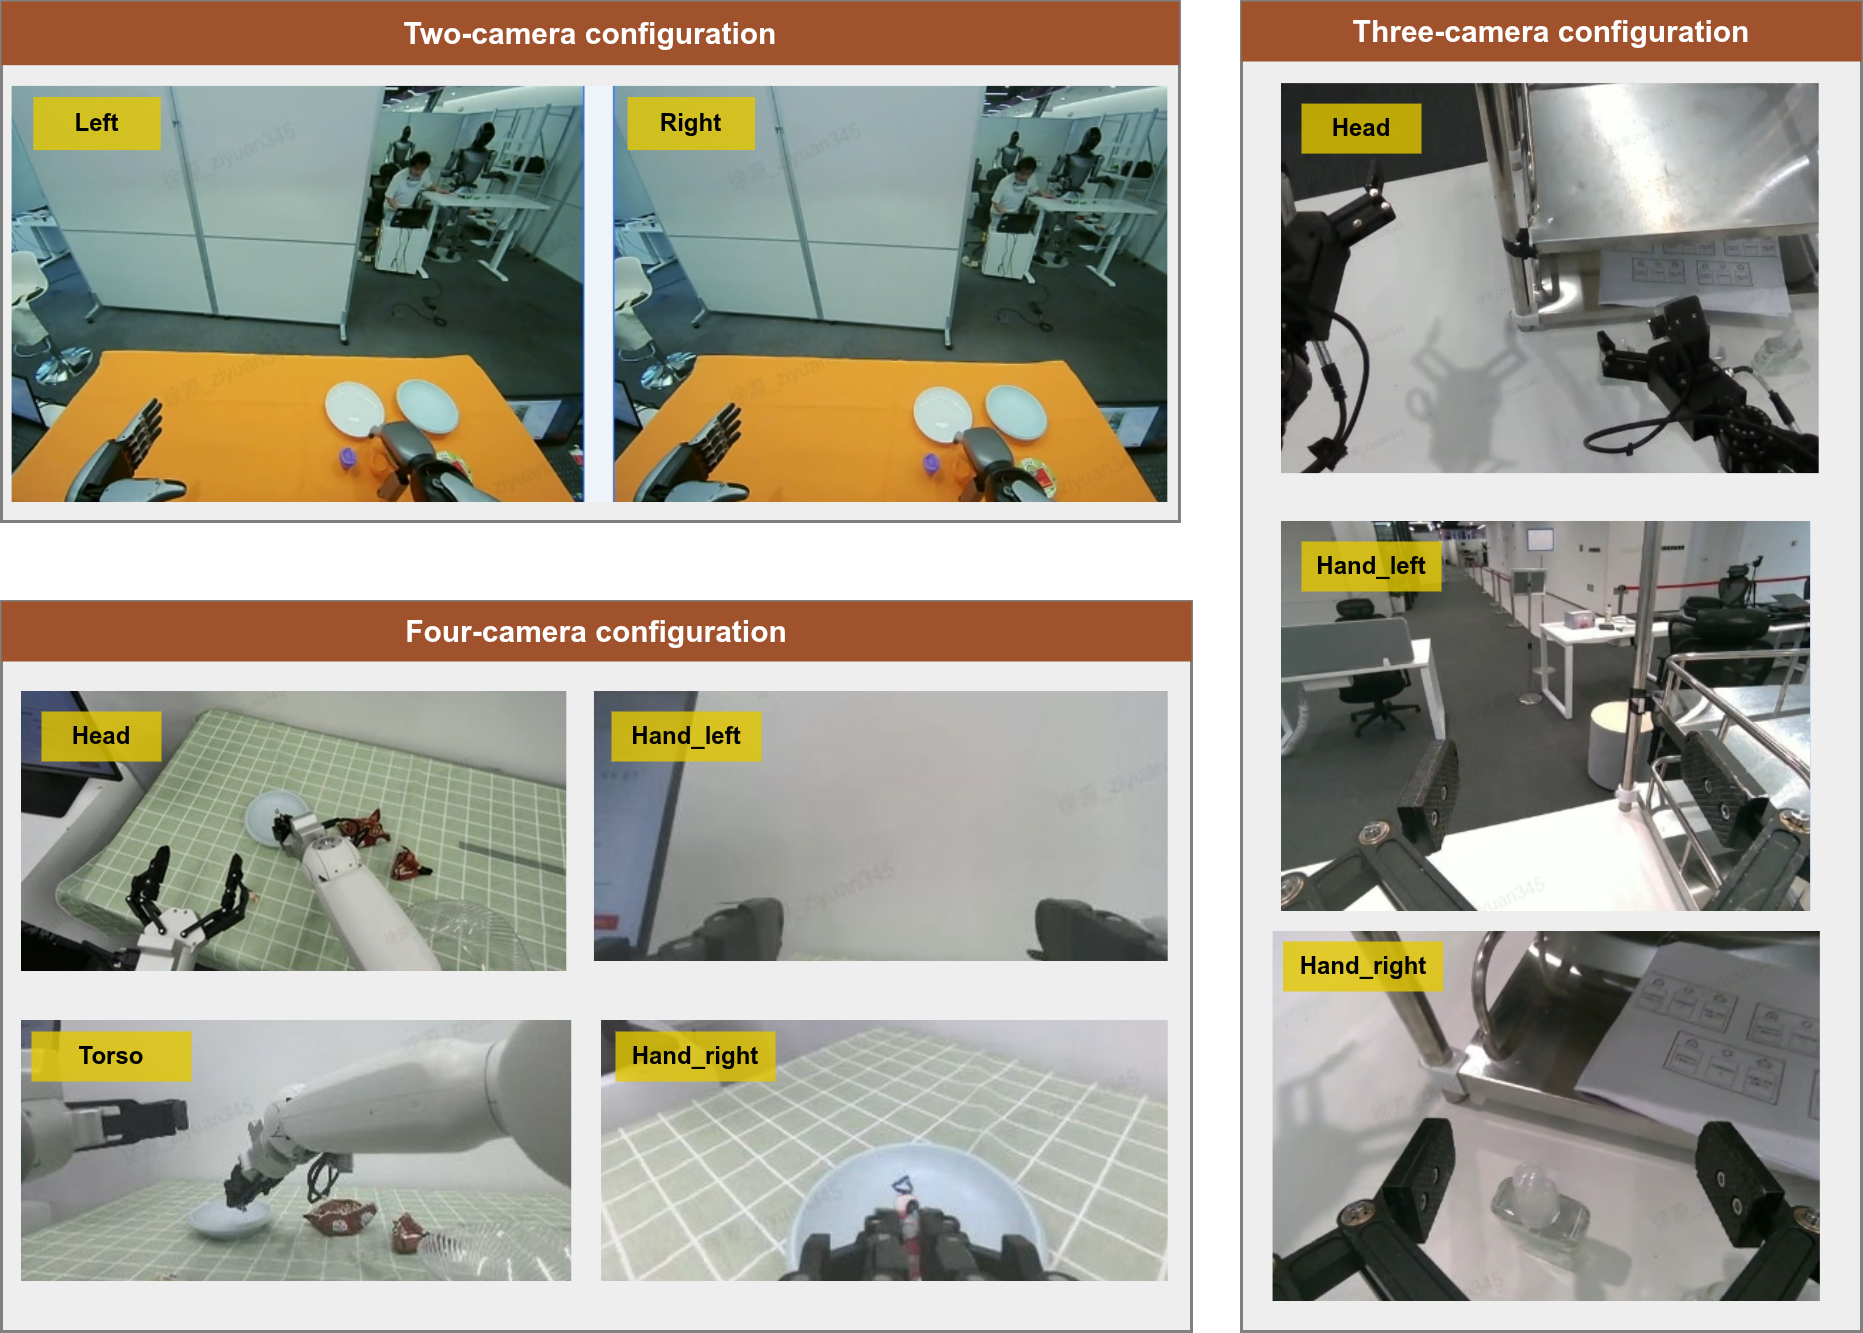
\includegraphics[width=\textwidth]{figures/相机视角.png}
\caption{Representative multi-camera visual observations in WhiteTiger, including a three-camera configuration on the left, a two-camera configuration in the upper right, and a four-camera configuration in the lower right. The examples illustrate view layouts without enumerating every platform or sensor configuration.}
\label{fig:camera-configurations}
\end{figure}

Morphology, visual viewpoint, end-effector type, and action dimensionality jointly determine the sensorimotor grounding available to a policy. WhiteTiger therefore uses platform-specific modality schemas within the shared LeRobot v2.1 representation rather than imposing a single universal observation-action layout.

\subsection{Object and interaction diversity}

WhiteTiger records interactions with household items, kitchen utensils, retail goods, packages, industrial parts, tools, flexible materials, and irregular objects. These objects vary in size, shape, material, rigidity, texture, and manipulation affordance. Object diversity is required for policies that must transfer beyond a fixed object inventory.

Interaction patterns include single-object pick-and-place, sorting, tool use, assembly-like manipulation, container interaction, drawer and door operation, and multi-object organization. These patterns impose different contact modes, spatial constraints, and failure conditions, supporting analysis of generalization across objects, tasks, environments, and physical interaction types.

\subsection{Data format}

WhiteTiger converts HDF5 source records into LeRobot v2.1. Each episode is represented as a temporally ordered trajectory of observation-action pairs. Depending on platform and task setup, a trajectory may contain visual observations, proprioceptive state, action commands, task labels, event annotations, timestamps, and episode metadata. The standardized format supports direct loading by robot learning pipelines and large-scale model training systems while retaining platform-specific observation and action schemas.

A typical trajectory contains a task instruction or task label, synchronized visual observations, robot proprioceptive states, robot actions, optional event records, episode metadata, and frame-level temporal ordering.

\subsection{Data availability}

Dataset access information, platform-specific modality definitions, event annotation schema, and benchmark resources will be provided through the official WhiteTiger repository. Licensing, permitted-use conditions, and access requirements will be documented with the released resources.
